\documentclass[11pt, a4paper]{article}

% --- UNIVERSAL PREAMBLE BLOCK ---
% Adjusted geometry for landscape slides as requested
\usepackage[landscape, top=1cm, bottom=1cm, left=1cm, right=1cm]{geometry}


% --- PACKAGES ---
\usepackage{tikz}
\usetikzlibrary{shapes.geometric, arrows.meta, positioning, calc, fit, backgrounds}

% --- UofSC COLOR DEFINITIONS ---
% Primary Colors
\definecolor{UofSCGarnet}{RGB}{115, 0, 10}
\definecolor{UofSCBlack}{RGB}{0, 0, 0}
\definecolor{UofSCWhite}{RGB}{255, 255, 255}

% Neutral Colors
\definecolor{UofSC90Black}{RGB}{54, 54, 54}
\definecolor{UofSC70Black}{RGB}{92, 92, 92}
\definecolor{UofSC50Black}{RGB}{162, 162, 162}
\definecolor{UofSC30Black}{RGB}{199, 199, 199}
\definecolor{UofSC10Black}{RGB}{235, 235, 235}
\definecolor{UofSCWarmGrey}{RGB}{103, 97, 86}
\definecolor{UofSCSandstorm}{RGB}{255, 242, 227}

% Accent Colors
\definecolor{UofSCRose}{RGB}{204, 46, 64}
\definecolor{UofSCAtlantic}{RGB}{70, 106, 159}
\definecolor{UofSCCongaree}{RGB}{31, 65, 77}
\definecolor{UofSCHorseshoe}{RGB}{101, 120, 11}
\definecolor{UofSCGrass}{RGB}{206, 211, 24}
\definecolor{UofSCHoneycomb}{RGB}{164, 145, 55}

% Special Use Colors
\definecolor{UofSCDarkGarnet}{RGB}{87, 0, 8}
\definecolor{UofSCAzalea}{RGB}{132, 66, 71}

\begin{document}

\begin{figure}[htbp]
\centering
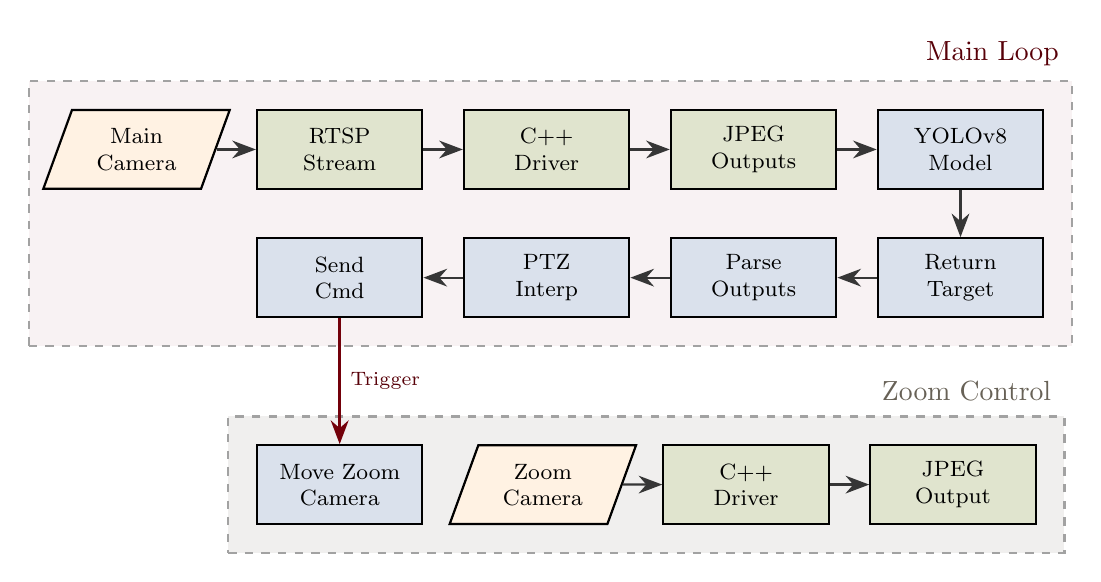
\begin{tikzpicture}[
    % Spacing
    node distance=0.6cm and 0.5cm,
    % --- STYLES MAPPED TO BRAND COLORS ---
    % Base: Dark Grey border, Sans Serif font
    base/.style={
        draw=UofSCBlack, 
        thick, 
        align=center, 
        font=\footnotesize
    },
    % Process: Default to very light grey
    process/.style={
        base, 
        rectangle, 
        minimum width=2.1cm, 
        minimum height=1cm, 
        fill=UofSC10Black
    },
    % Logic: Mapped to Atlantic (Blue) - Light tint
    logic/.style={
        base, 
        rectangle, 
        minimum width=2.1cm, 
        minimum height=1cm, 
        fill=UofSCAtlantic!15
    },
    % IO: Mapped to Sandstorm (Tan/Orange substitute)
    io/.style={
        base, 
        trapezium, 
        trapezium left angle=70, 
        trapezium right angle=110, 
        minimum width=2.1cm, 
        minimum height=1cm, 
        fill=UofSCSandstorm
    },
    % Drivers: Mapped to Horseshoe (Green substitute) - Light tint
    driverstyle/.style={
        process,
        fill=UofSCHorseshoe!20
    },
    % Python Logic: Mapped to Atlantic (Blue) - representing Python code
    pythonstyle/.style={
        process,
        fill=UofSCAtlantic!20
    },
    % Arrows: Dark Garnet for visibility
    arrow/.style={
        thick, 
        color=UofSC90Black,
        -{Stealth[length=3mm]}
    },
    % Groups: Dashed lines
    group/.style={
        draw=UofSC50Black, 
        dashed, 
        thick, 
        inner sep=10pt
    }
]

% --- 1. MAIN DETECTION LOOP (Snake Layout) ---

% Row 1: Left to Right
\node (camera) [io] {Main\\Camera};
\node (rtsp) [driverstyle, right=of camera] {RTSP\\Stream};
\node (driver) [driverstyle, right=of rtsp] {C++\\Driver};
\node (jpeg) [driverstyle, right=of driver] {JPEG\\Outputs};
\node (yolo) [pythonstyle, right=of jpeg] {YOLOv8\\Model};

% Row 2: Right to Left (Directly below Row 1)
\node (return) [pythonstyle, below=of yolo] {Return\\Target};
\node (parse) [pythonstyle, left=of return] {Parse\\Outputs}; 
\node (ptz) [pythonstyle, left=of parse] {PTZ\\Interp};
\node (cmd) [pythonstyle, left=of ptz] {Send\\Cmd};


% --- 2. INDEPENDENT ZOOM THREAD ---
% Starts below 'Send Cmd' and flows Left to Right

\node (movezoom) [pythonstyle, below=of cmd, yshift=-1cm] {Move Zoom\\Camera};
\node (zoomcam) [io, right=of movezoom] {Zoom\\Camera};
\node (zoomdriver) [driverstyle, right=of zoomcam] {C++\\Driver};
\node (zoomjpeg) [driverstyle, right=of zoomdriver] {JPEG\\Output};


% --- CONNECTIONS ---

% Main Pipeline (Row 1)
\draw [arrow] (camera) -- (rtsp);
\draw [arrow] (rtsp) -- (driver);
\draw [arrow] (driver) -- (jpeg);
\draw [arrow] (jpeg) -- (yolo);

% Loop Back (Row 1 End to Row 2 Start)
\draw [arrow] (yolo.south) -- (return.north);

% Main Pipeline (Row 2)
\draw [arrow] (return) -- (parse);
\draw [arrow] (parse) -- (ptz);
\draw [arrow] (ptz) -- (cmd);

% Connection to Zoom Thread
% Using Garnet here to emphasize the Trigger action
\draw [arrow, color=UofSCGarnet, very thick] (cmd.south) -- node[midway, right, font=\scriptsize, color=UofSCDarkGarnet] {Trigger} (movezoom.north);

% Zoom Thread Flow
\draw [arrow] (zoomcam) -- (zoomdriver);
\draw [arrow] (zoomdriver) -- (zoomjpeg);


% --- GROUPS ---

\begin{scope}[on background layer]
    % Main Loop Box - Garnet Tint
    \node [group, fit=(camera) (yolo) (cmd) (return), fill=UofSCGarnet!5, label={[anchor=south east, inner sep=5pt, color=UofSCDarkGarnet]north east:Main Loop}] {};
    
    % Zoom Thread Box - Warm Grey Tint
    \node [group, fit=(movezoom) (zoomjpeg), fill=UofSCWarmGrey!10, label={[anchor=south east, inner sep=5pt, color=UofSCWarmGrey]north east:Zoom Control}] {};
\end{scope}

\end{tikzpicture}
\end{figure}

\end{document}